\documentclass[a4paper,10pt]{article}
\usepackage[utf8]{inputenc}
\usepackage{hyperref}
\usepackage{graphicx}
\usepackage{amssymb}
\usepackage{amsmath}
\usepackage[margin=0.7in]{geometry}

\title{Building a Granular Dataset of UK Companies}
\author{Alfred Holmes}


\date{September 2018}
\begin{document}
   \maketitle
   \begin{abstract}
   The UK government, through the Office for National Statistics and Companies House release detailed data on UK companies. Using this publicly available data, it is possible to track the location and assets of companies through time and using few assumptions assign employment sizes to these companies and reproduce ONS reported statistics. This report summaries the available data and details the use of the data to compile a granular dataset.
   \end{abstract}
   \section{Introduction}
   To use contemporary techniques to model the UK economy, a detailed granular dataset of UK companies is required. Ideally the dataset would contain the employment size and turnover evolution of each company, as well as the location and number of employees of individual branches through time. From this, one could easily generate a detailed picture of the UK economy and it's evolution.
   \subsection{Definitions}
   These definitions are used consistently throughout this document, and provide clarity when describing subtly different entities.
   \begin{itemize}
 	\item Company - an entity registered on Companies House. In June 2017 there were 3.1 million registered companies in the UK. 
 	\item Enterprise - a business that is reported by ONS. We assume that an enterprise is a collection of companies. In 2017 the ONS reported 2.7 million enterprises.
 	\item Local Authority - a connected area of land the UK governed by a council. In June 2017, local authorities have a population of 170 000 people and 7 000 enterprises on average. There are 391 local authorities in the UK.
   \end{itemize}

   \section{Available Data}
   The UK government through Companies House and the Office for National Statistics release detailed data on UK businesses. All data used in this study is provided through the Open Government License.
   \subsection{Companies House}
   Companies House is the public service responsible for incorporating and dissolving companies in the UK, as well as storing and releasing company data. They provide monthly snapshots of basic company information, all the online accounts that have been filed since 2008 and also provide an API where more detailed information - changes of address and people of significant control - can be accessed on a company by company basis.
   \subsubsection{Snapshots}
   The companies house snapshots \cite{companieshousesnapshots} are only available for the current month and only contain active companies and don't contain data on the history of each company. Luckily \emph{webarchive} \cite{snapshotarchive} has archived approximately 1 snapshot per year, so this can be used to get low resolution historic data for companies. 
   \subsubsection{Accounts}
   If a company files its accounts online then that account filing is available to download through the companies house accounts data product \cite{accountsdataproduct}. This means that for increasingly many companies detailed financial data is available.
   The files are given as one XML (or HTML) file per account file per company per year. The most effective way to read these files is to recursively see if there is a number between two tags and if there is pull the number, its title and date. The \texttt{data/accounts} folder in the GitHub repository \cite{github} contains useful python scripts to process the accounts data. The following table summarises the available accounts data. The percentages proportion of accounts that contain the heading. There is a high correlation between having one of the heading and having the other. The ratio of filed accounts of active companies to active companies increases from 35\% in 2008 to about 60\% in 2017.
   \begin{center}
      \begin{tabular}{  c | c | c | c  }
      Year & Number of Accounts & netcurrentassetsliabilities & currentassets \\
      \hline
      2008 & 185163  & 59\% & 58\% \\
      2009 & 344403  & 64\% & 63\% \\
      2010 & 585143  & 71\% & 70\% \\
      2011 & 793218  & 74\% & 73\% \\
      2012 & 1033277 & 76\% & 74\% \\
      2013 & 1219357 & 77\% & 71\% \\
      2014 & 1573870 & 77\% & 72\% \\
      2015 & 1811446 & 77\% & 72\% \\
      2016 & 2071697 & 78\% & 72\% \\
      2017 & 2324272 & 79\% & 73\% \\
      \end{tabular}
   \end{center}


   \subsubsection{Companies House API}
   The Companies House API \cite{companieshouseapi} can be used to get detailed information about a company given its name or company number. The API has a request limit of 2 requests per second per API key, so to make one query per company for all companies registered since 2012 it would take 32 days. The service does allow multiple API keys to be registered which can speed up data acquisition. The API can be used to get all the filings for a particular company, with the exact dates of each. See the folder \texttt{data/API} in \cite{github} for a script that pulls the changes of address for companies.
   \subsection{Office for National Statistics}
   \subsubsection{Business Activity, Size and Location}
   \label{basl}
   The Business Activity, Size and Location tables from the ONS \cite{basl}, available for 2012 to 2017, report by local authority and SIC code, the number of enterprises with size in a particular range. For example, for employment statistics the ONS typically give the number of enterprises with employees in the ranges \emph{0-4, 5-9, 10-19, 20-49, 50-99, 100-249} and \emph{250+}. The turnover is treated similarly.
   
   \subsubsection{Postcode Data}

   Since the data by location in \ref{basl} is by local authority, a useful resource is the postcode lookup tables \cite{postcodes}. These tables allow addresses of individual companies to be matched to local authorities. Included in the folder \texttt{useful} in \cite{github} is a slimmed down postcode table with just the postcode and its associated local authority's id as well as \texttt{lad\_17\_geo\_info.csv} which is a collection of the possible names on ONS documents and region information for each local authority\footnote{Local authority names sometimes have different spellings / word orders in different ONS datasets}.

   \subsubsection{Employment}

   The ONS also report employment \cite{employment} by location and also by SIC code broken down into public and private sector jobs. We assume that all the companies listed on companies house are private entities, and hence any employees are working in the private sector. The employment is useful as it allows the mean company size to be calculated.

   \section{Issues Combining ONS and Companies House data}


   \subsection{Number of Companies}
   \label{company_enterprise_error}

   \begin{figure}[h]
      \begin{center}
         \caption{Total Number of Companies registered on Companies House and reported by ONS}
         \label{ch_vs_ons}
         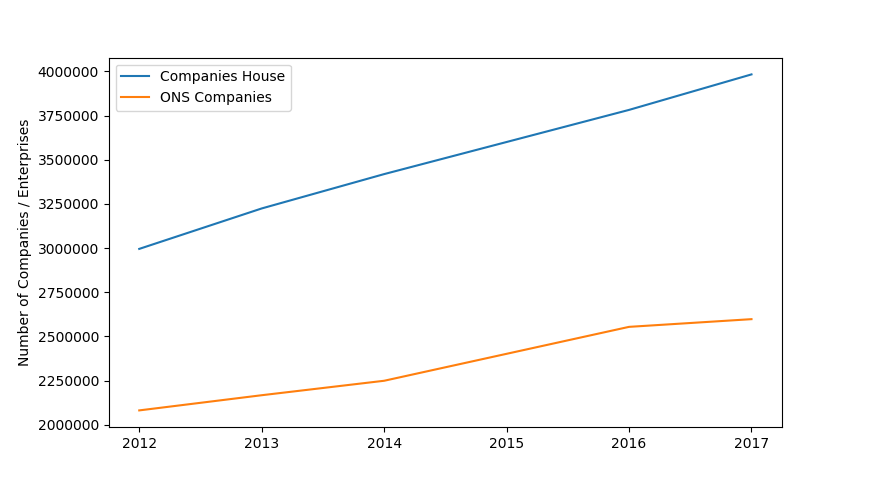
\includegraphics[width=12cm]{graphs/companies_house_vs_ons/companies_house_vs_ons}
      \end{center}
   \end{figure}
   % TODO: Removing repeated addresses for offices

   Looking at figure \ref{ch_vs_ons} it is clear that an ONS enterprise isn't just a companies house company. This is because many enterprises are made up of multiple companies. Because of this issue, for this report we assume that if two companies share the same set of addresses then they are part of the same enterprise. This reduces the error between the companies, but there is still a large difference between the number of companies and enterprises. Due to this issue, we will use proportions in this report rather than actual numbers of companies and enterprises.

   \subsection{SIC Codes}

   Companies House companies can have multiple SIC codes and also have 5 digit SIC codes. The ONS reports contain the number or enterprises with a particular 4 or 2 digit SIC code. It is not clear how they decide which SIC code to give to a particular enterprise, but it it likely that the enterprise give the SIC code in response to a survey. This means that it is difficult to infer the SIC code from an enterprise's companies. For this reason, the number of enterprises with a 4 digit SIC code given by ONS does do not form a strong linear relationship with that inferred from the companies house data. The 2 digit SIC codes are better because if a company reports two SIC codes, then it is likely that are in the same broad industry group and so they share the first two digits.

   \section{Fitting Lognormal Distributions}
   To make the ONS data usable some sort of size distribution needs to be assumed. This is not ideal since there are many different factors going in to company growth that can't be captured by simple growth models. Using Maximum Likelihood Estimation (MLE) and the ONS size bins as well as the mean company sizes, it is possible to fit distributions to the data. This has two benefits in that it assigns the mass of the probability distribution in a band in a sensible way and also removes the irritating \emph{250+} size band.
   
   \subsection{MLE}
  
   Assuming a lognormal distribution where the size X of a company is such that $\log X \sim \mathcal{N}(\mu, \sigma^2)$, $\mu$ and $\sigma$ can be estimated by maximising the log likelihood, given by
   \begin{equation}
   l(\mu, \sigma) = \sum_i n_i \log \left( \Phi \left( \frac{\log a_{i + 1} - \mu}{\sigma} \right) - \Phi \left( \frac{\log a_{i} - \mu}{\sigma} \right) \right)
   \end{equation}
   since $\mathbb{P}(a_i < X < a_{i + 1}) = \mathbb{P}(\log a_i < \log X < \log a_{i + 1}) = \Phi \left( \frac{\log a_{i + 1} - \mu}{\sigma} \right) - \Phi \left( \frac{\log a_{i} - \mu}{\sigma} \right)$. \\
 For local authority and country wide parameter fitting, the total private employment, $e$, is released by ONS. From this, as the number of companies, $n$, is known the mean of the distribution can be used to constrain the parameters such that $\mu$ and $\sigma$ satisfy the equation $\exp(\mu + \frac{\sigma^2}{2}) = \frac{e}{n}$ in order to reduce the error of the predictions.

   \subsubsection{Simulations}

   In order to test whether the MLE can recover the distribution parameters from the size bins we ran simulations: picking random numbers from a known distribution and then trying to recover the distribution parameters. In this section we focus on recovering the employment parameters, so use parameters which generate distributions that fill the ONS enterprise sizes size bins. For these simulations we assume that the number of enterprises is large enough that the number in each bin is close to the expected value. The python scripts for these simulations can be found in the \texttt{Lognormal Bias} folder in \cite{github}. Running the script \texttt{analysis.py} gives an interactive version of the 3D graphs in figure \ref{bias}.


   \begin{figure}[!ht]
      \begin{center}
         \caption{Simulated Bias. The spikes are due to the binned data being ambiguous - at least two sets of parameters lead to the observed binned distribution and the MLE picks different parameters.}
         \label{bias}
         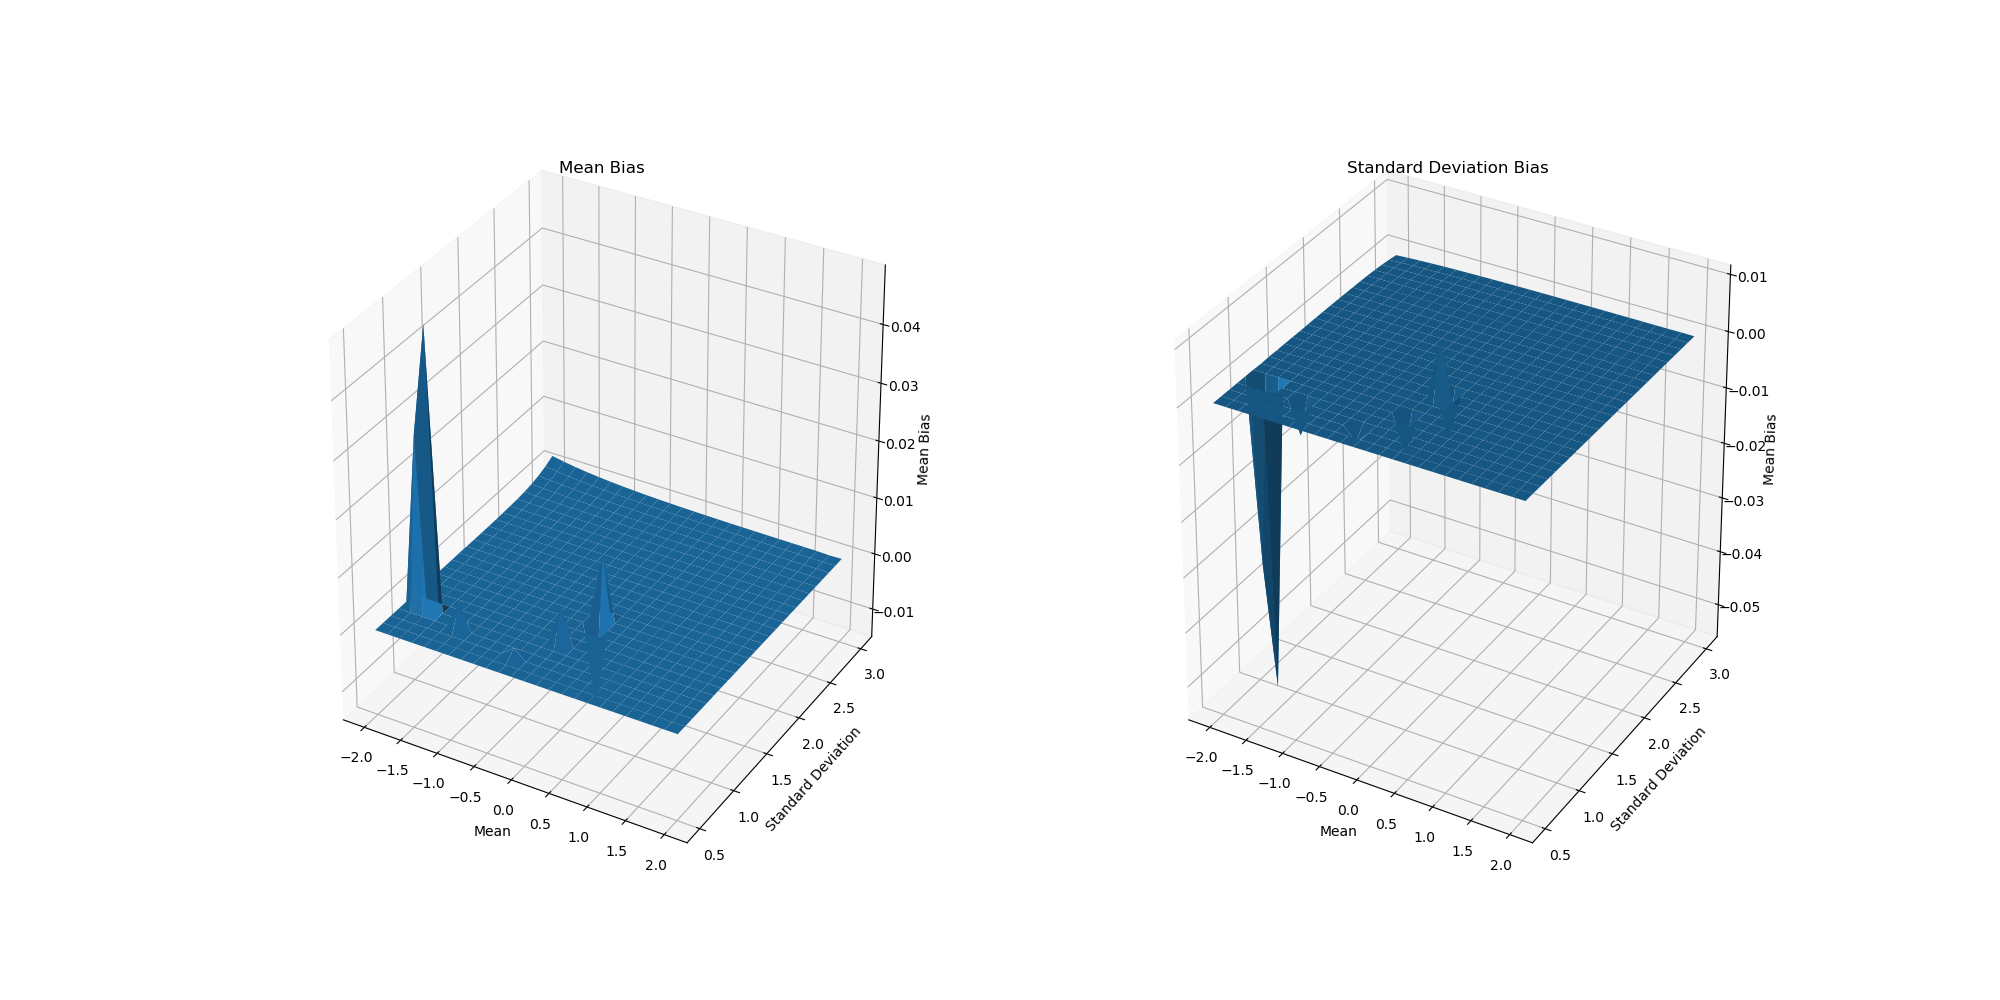
\includegraphics[width=\textwidth]{graphs/bias}
      \end{center}
   \end{figure}
   Figure \ref{bias} shows that the parameter estimation generally works quite well for the typical parameters in the observed distributions. In order to test the fit of the fitted parameters, we estimate the parameters from the ONS binned data and then use the distribution parameters to calculate the expected proportion of companies with in each bin and then plot those proportions. Although not the most mathematically rigorous method, this is a quick way to get a clear picture about the parameter estimation.
   \begin{figure}[!ht]
      \begin{center}
         \caption{Plot to evaluate parameter estimation. 100 points plotted with $(\mu, \sigma) \in [-1, 1] \times [0.5, 3]$. The left plot contains 7 points for each parameter pair, and the right plot is of the same data but connecting each set of points.}
         \label{parameter_reconstruction}
         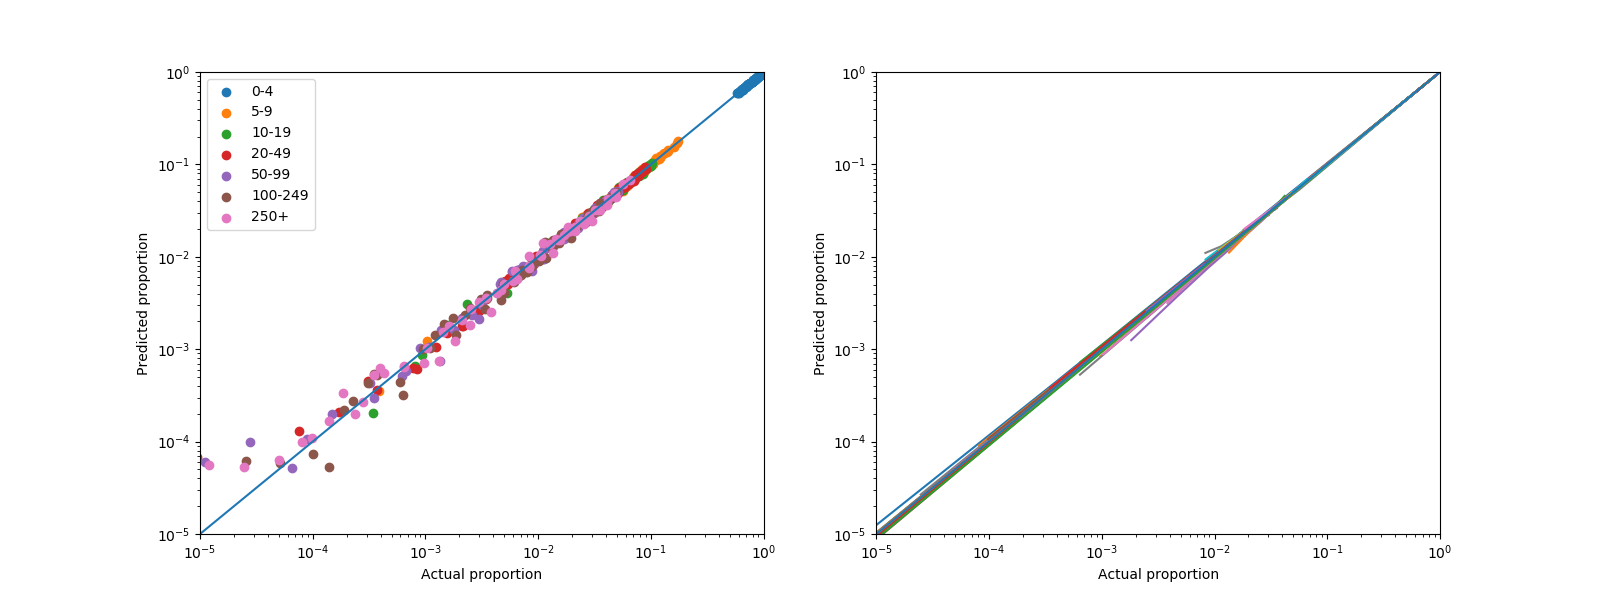
\includegraphics[width=\textwidth]{graphs/loglog_reconstruction}
      \end{center}
   \end{figure}

	The results in figure \ref{parameter_reconstruction} show that if the size distribution of companies is approximately log normal then using the available ONS data, it is possible to recover the parameters of the underlying distributions.

   \subsubsection{Matching Enterprise Employment}
   \label{enterprise_employment}
   The same procedure can then be applied to the ONS data. Figure \ref{2014_size_dist_results} indicates that although the underlying distribution of enterprise sizes is not lognormal, the fitted distribution does an adequate job of predicting the enterprise sizes.

   \begin{figure}[!ht]
      \begin{center}
         \caption{2014 ONS Employment size. Each point represents a size bin of a local authority.}
         \label{2014_size_dist_results}
         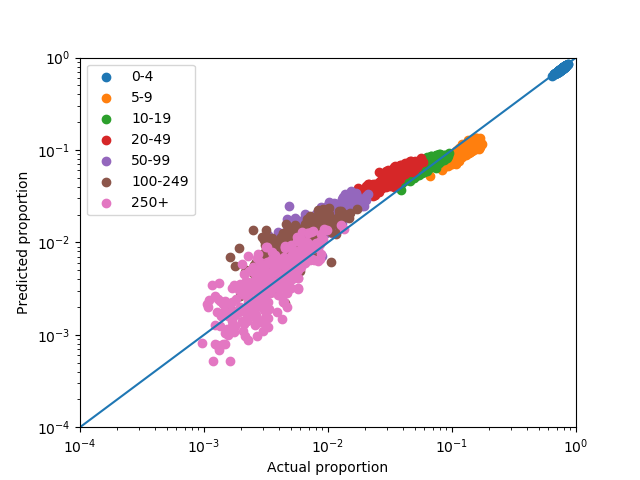
\includegraphics[width=10cm]{graphs/2014_enterprise_size_by_la}
      \end{center}
   \end{figure}


   \label{enterprise_employment}
   \section{Assigning Sizes to Enterprises}
   \label{assigning_sizes}
   For this section we will focus on the year 2014. The same approach can be used for all the other years in the sample. To assign employment size to enterprises we assume the following:
   \begin{itemize}
      \item Companies who do not report their accounts have assets of 0 value.\footnote{This assumption is made since when processing the data it is difficult to distinguish whether a company did not report assets or is exempt from reporting the data due to being small.}
      \item If company $a$ has more assets than company $b$ and $a$ and $b$ have the same SIC code, then company $a$ employs more people than company $b$.
   \end{itemize}



   We then pull $n$ numbers from the fitted lognormal distribution of company sizes for each SIC code, where $n$ is the number of companies with each SIC Code, and sort the list. We then sort the companies by asset size and assign size $i$ to company $i$. Using the same technique as in \ref{enterprise_employment} we then plot the predictions (figure \ref{enterprise_employment_reconstruction_using_sic}).
  	\begin{figure}
      \begin{center}
         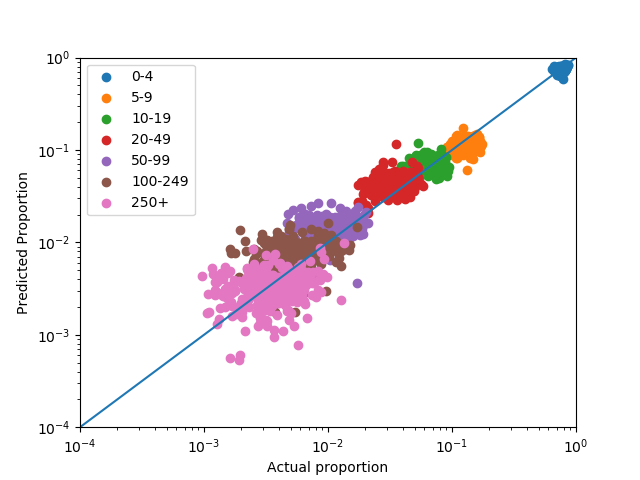
\includegraphics[width=10cm]{graphs/2014_la_reconstruction}
         \caption{Local Authority Employment Reconstruction using SIC code distributions}
         \label{enterprise_employment_reconstruction_using_sic}
      \end{center}
   \end{figure}


   \subsection{Evaluating the the assigned sizes}

   One simple test and use for the data set is to try and reproduce the ONS reported private employment rates. To do this we use the sizes generated using the SIC code distributions and add up the enterprise sizes. Due to the issues raised in section \ref{company_enterprise_error}, we test the employment predictions by looking at the ratios of total employment, rather than plotting absolute employment statistics.

  	\begin{figure}
      \begin{center}
         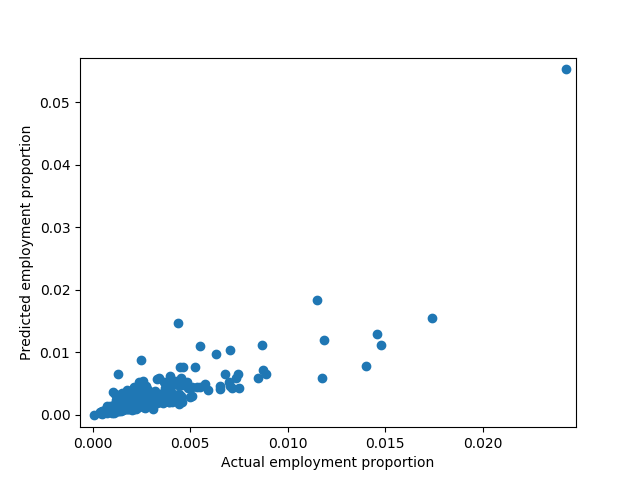
\includegraphics[width=9cm]{graphs/employment_prediction_with_london}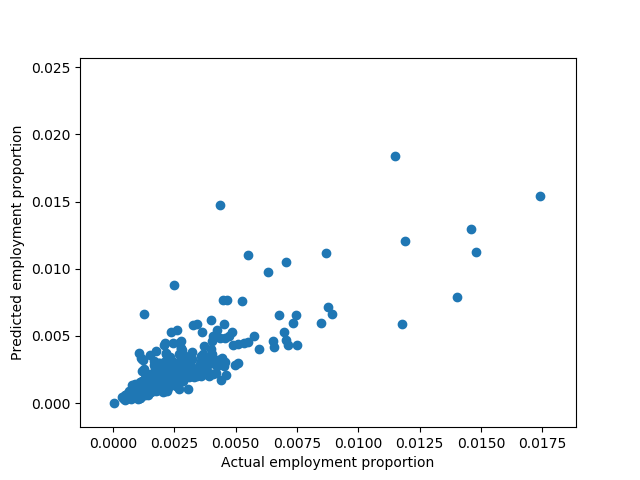
\includegraphics[width=9cm]{graphs/employment_prediction}
         \caption{Local Authority Employment Reconstruction using SIC code distributions. The right is a zoomed in version of the left}
         \label{employment_predictions}
      \end{center}
   \end{figure}


   We see in figure \ref{employment_predictions} that the employment predictions are reasonable - with a gradient of approximately 1. There is a fair amount of error in the data but this is to be expected, as the prediction assumes that all the workers for a company work in that companies registered office location, which is not true for many jobs. This is seen in the outlier, Westminster, since central London is a common place for large company headquarters with companies such as \emph{Marks and Spencer}\cite{companieshousesnapshots}.
   

   \section{Improvements}

   To improve this dataset the most important issue to sort out is the issue discussed in section \ref{company_enterprise_error} since this would allow a much finer understanding of how the ONS data relates to the companies house entities. We found that if the assumption that all enterprises with a given SIC code, $s$, have a probability, $p_s$, of having a companies house registered enterprise (set of companies with the same set of addresses) is made then by finding $p_s$ for each $s$ we could improve the predictions. The problem with this approach is that it creates two granular sets of enterprises, the ones from companies house and the set with the correct number of companies, and it is difficult to use the companies house data to then infer the properties of the second set without making untestable assumptions.

   Another important improvement would be to map and assign branches to companies. ONS release data on the number and size of local units in each local authority, so this could be used to assign branches and associated employees to enterprises. Since the technique for assigning employees to enterprises in section \ref{assigning_sizes} doesn't use the location of the company, there are no ties for the employees of an enterprise registered in a particular local authority to work there. From the ONS reports, it is not clear how the location of an enterprise is assigned - whether it is the registered office address of the enterprise, or where the company is acting. A clever assignment of branches to the enterprises would allow the size assignations to predict employment accurately and also track the flow of employment around the UK using the companies house migration data.

   \medskip


   \begin{thebibliography}{9}
      \bibitem{companieshousesnapshots}
      Companies House Snapshot: list of basic company information for the current month's UK registered active companies
      \\\texttt{http://download.companieshouse.gov.uk/en\_output.html}

      \bibitem{snapshotarchive}Companies House Snapshot Archive
      \\\texttt{https://web.archive.org/web/20120901000000*/http://download.companieshouse.gov.uk/en\_output.html}

      \bibitem{accountsdataproduct}
      Accounts Data Product
      \\\texttt{http://download.companieshouse.gov.uk/historicmonthlyaccountsdata.html}
      
      \bibitem{github}
      UK Company Data GitHub repository
      \\\texttt{http://github.com/alfredholmes/uk-company-data}

      \bibitem{companieshouseapi} 
      Companies House API
      \\\texttt{https://developer.companieshouse.gov.uk/api/docs/}

      \bibitem{basl}
      Business Activity Size and Location
      \\2012:
      \\\texttt{http://webarchive.nationalarchives.gov.uk/20140511113648/http://www.ons.gov.uk/ons/publications/\\re-reference-tables.html?edition=tcm\%3A77-254601\&format=hi-vis}
      \\2013:
      \\\texttt{http://webarchive.nationalarchives.gov.uk/20140510023623/http://www.ons.gov.uk/ons/publications/\\re-reference-tables.html?edition=tcm\%3A77-313744\&format=hi-vis}
      \\2014 - 2017:
      \\\texttt{https://www.ons.gov.uk/businessindustryandtrade/business/activitysizeandlocation/datasets/\\ukbusinessactivitysizeandlocation}
      
      
      \bibitem{employment}
      ONS Employment Statistics
      \\\texttt{https://www.ons.gov.uk/employmentandlabourmarket/peopleinwork/employmentandemployeetypes/\\datasets/summaryoflabourmarketstatistics/current}

      \bibitem{postcodes}
      ONS Postcode Data
      \\\texttt{http://geoportal.statistics.gov.uk/datasets/postcode-to-output-area-to-lower-layer-super-output\\-area-to-middle-layer-super-output-area-to-local-authority-district-august-2018-lookup-in-the-uk}

   \end{thebibliography}








\end{document}